%%%%%%%%%%%%%%%%%%%%%%%%%%%%%%%%%%%%%%%%%
% Beamer Presentation
% LaTeX Template
% Version 1.0 (10/11/12)
%
% This template has been downloaded from:
% http://www.LaTeXTemplates.com
%
% License:
% CC BY-NC-SA 3.0 (http://creativecommons.org/licenses/by-nc-sa/3.0/)
%
%%%%%%%%%%%%%%%%%%%%%%%%%%%%%%%%%%%%%%%%%

%----------------------------------------------------------------------------------------
%	PACKAGES AND THEMES
%----------------------------------------------------------------------------------------

\documentclass{beamer}

\mode<presentation> {
\usetheme{Madrid}
\usefonttheme{serif} 
\setbeamertemplate{navigation symbols}{} % To remove the navigation symbols from the 
}
\usepackage{lmodern}  
\usepackage{graphicx} % Allows including images
\usepackage{booktabs} % Allows the use of \toprule, \midrule and \bottomrule in tables
\usepackage[T1]{fontenc}
\usepackage[utf8]{inputenc}
\usepackage{amsmath}
\usepackage{color}
\usepackage[czech]{babel}
\usepackage{lmodern}  
\usepackage{rotating}
\usepackage{scrextend}
\usepackage{pifont}
\usepackage{hyperref}
\usepackage{bm}
\usepackage{tikz}%boxy  
\usetikzlibrary{arrows,positioning}
\usetikzlibrary{calc}
%
\newcommand*\circled[1]{\tikz[baseline=(char.base)]{
    \node[shape=circle,draw=red,inner sep=2pt] (char) {#1};}}
%
\newcommand*\circledd[1]{\tikz[baseline=(char.base)]{
    \node[shape=circle,draw=ProcessBlue, dashed, inner sep=2pt] (char) {#1};}}
%
\newcommand{\mytikzmark}[2]{%
  \tikz[remember picture,inner sep=0pt,outer sep=0pt,baseline,anchor=base] 
    \node (#1) {\ensuremath{#2}};}
%
%
\newcommand*{\boxcolor}{Red}
\makeatletter
\renewcommand{\boxed}[1]{\textcolor{\boxcolor}{%
\tikz[baseline={([yshift=-1ex]current bounding box.center)}] \node [rectangle,semithick, minimum width=1ex,draw, dashed] {\normalcolor\m@th$\displaystyle#1$};}}
 \makeatother
%
%----------------------------------------------------------------------------------------
%	TITLE PAGE
%----------------------------------------------------------------------------------------
\title[Block 6]{Praktikum z ekonometrie} % The short title appears at the bottom of every slide, the full title is only on the title page
\author{VŠE Praha} % Your name
\institute[4EK417] % Your institution as it will appear on the bottom of every slide, may be shorthand to save space
{
% Your institution for the title page
\medskip
\textit{Tomáš Formánek} % Your email address
}
\date{} % Date, can be changed to a custom date
%----------------------------------------------------------------------------------------
\begin{document}
\begin{frame}
\titlepage % Print the title page as the first slide
\end{frame}
%---------------------------------------------------------------------
\begin{frame}
\frametitle{Block 6 – Treatment effects – Outline
} % Table of contents slide, comment this block out to remove it
\tableofcontents % Throughout your presentation, if you choose to use \section{} and \subsection{} commands, these will automatically be printed on this slide as an overview of your presentation
\end{frame}

%----------------------------------------------------------------------------------------
%	PRESENTATION SLIDES
%---------------------------------------------------------------------
\section{Treatment effects: Introduction}
\begin{frame}{Treatment effects: Introduction}
\begin{itemize}
    \item Evaluation focuses on the impact of intervention (treatment) on some \textbf{outcome} of interest.
    \medskip
    \item We are interested in measuring response to treatment. Such response is evaluated relative to a benchmark: no treatment or different treatment. 
    \medskip
    \item \textbf{Outcome} typically refers to (changes in)  `status' (economic, social, medical, etc.) of individuals / companies / CS units.
    \medskip
    \item Analysis of treatment effect is typically based on regression models, with \textbf{outcome} as the dependent variable.
\end{itemize}
\end{frame}
%---------------------------------------------------------------------
\begin{frame}{Treatment effects: Introduction}
\textbf{Examples of treatment} in the socio-economic context \\ \medskip
\begin{itemize}
    \item Enrollment in some form of labor training program
    \medskip
    \item Becoming member of trade union
    \medskip
    \item Receiving transfer payment from a social program
    \medskip
    \item Changes in regulations (imposing/alleviating restrictions)
    \medskip
    \item Being educated in small classes (as opposed to large classes) 
\end{itemize}
\bigskip
\textbf{Multiple treatments:} If treatment can vary in intensity or type. Comparing a single type of treatment to benchmark does not add complexity, yet the choice of benchmark is more flexible.
\end{frame}
%---------------------------------------------------------------------

% Define box and box title style
\tikzstyle{mybox} = [draw=blue!35, fill=white, very thick,
    rectangle, rounded corners, inner sep=1pt, inner ysep=10pt]
\tikzstyle{fancytitle} =[fill=blue!35, text=black]
%---------------------------------
\begin{frame}{Treatment effects: Introduction}
\textbf{Studies of treatment effects:} types of studies and types of data used for evaluation:\\
\begin{itemize}
    \item ``Proper'' (controlled) scientific experiments: assignment into treated and control groups is random. \\ \medskip Relatively rare in socio-economic studies (common/required in medical studies, etc.). 
    \bigskip
    \item Observational studies -- natural experiments, quasi-experiments (assignment into treatment and control group is not random) \\ \medskip
    
    Self-selection bias (treatment participation is optional, individuals who choose to participate may be systematically different from non-participant)
\end{itemize}
\end{frame}
%---------------------------------
\begin{frame}{Treatment effects: Introduction}
\begin{tikzpicture}
\node [mybox] (box){%
\begin{minipage}{0.50\textwidth}
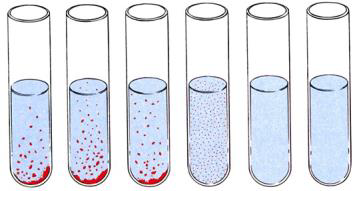
\includegraphics[width=\textwidth, height=2.89cm]{./IMG/Obrazek1}
\begin{itemize}
\scriptsize
\item Test tubes identical except for catalyst
\item Measure: Effect at different catalyst volumes (reaction speed, product volume, \dots)
\item Perform the experiment $n$-times
\item Control for other factors (heat, \dots)
\item Estimate average effect \\(\& standard error)
\end{itemize}
\end{minipage}
};
\node[fancytitle, right=5pt,  rounded corners] at (box.north west) {\scriptsize Scientific experiment};
\end{tikzpicture}%
\begin{tikzpicture}
\node [mybox] (box){%
\begin{minipage}{0.50\textwidth}
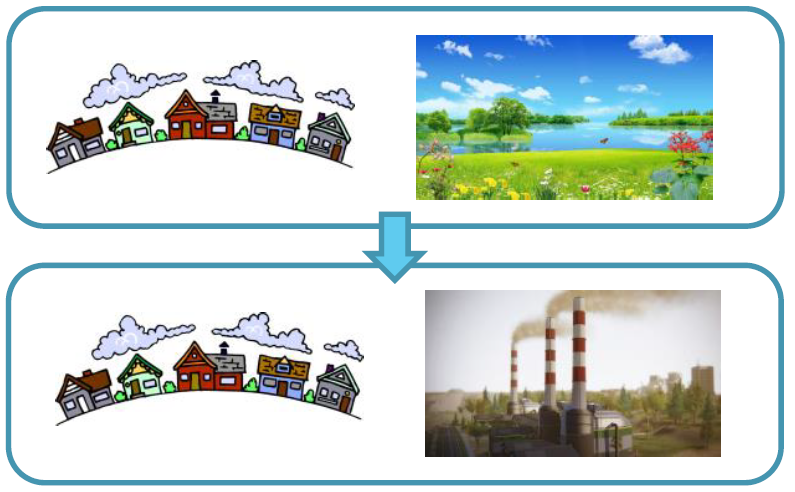
\includegraphics[width=\textwidth]{./IMG/Obrazek2}
\begin{itemize}
\scriptsize
\item Garbage incinerator is built in one given
suburban area over time
\item How do we estimate the effect on
individual house-prices?
\item Identical control group does not exist…
\item Different estimators exist\\
(assumptions apply!)
\end{itemize}
\end{minipage}
};
\node[fancytitle, right=5pt,  rounded corners] at (box.north west) {\scriptsize Natural experiment (quasi-experiment)};
\end{tikzpicture}%
\end{frame}
%---------------------------------
\begin{frame}{Treatment effects: Introduction}
\small
For evaluation of scientific experiments (if treatment/intervention is exogenous), one can formulate a regression model with a treatment-related dummy variable, as follows:
$$
y_i = \bm{x}_i^{\prime}\bm{\beta} + \delta D_i + \varepsilon_i,
$$
where $D_i = 1$ if the $i$th individual (CS unit) is in the treatment group and zero otherwise (for the control group). \\
\medskip
For a simplified scenario, we can leave out covariates $\bm{x}$ and compare two groups (treated/untreated):
$$
y_i = \beta_0 + \delta D_i + \varepsilon_i,
$$    
with $\hat{\beta}_0 = [\overline{y}|_{D_i=0}]$ being the average outcome for the untreated,\\
and $\hat{\delta} = [\overline{y}|_{D_i=1}] - [\overline{y}|_{D_i=0}]$ as the mean difference between the two groups.\\
\bigskip
\textbf{Note:} exogeneity of $D$ is crucial for estimation of the treatment effect. Inclusion of $\bm{x}_i^{\prime}\bm{\beta}$ in the equation doesn't change the general interpretation of $\delta$.
\end{frame}
%---------------------------------
\section{DiD estimator: Policy analysis with pooled CS data}
\begin{frame}{DiD estimator: Policy analysis with pooled CS data} 
\small
DiD refers to a popular approach towards policy analysis \& evaluation, based on models with two dummy variables: $T$ differentiates between two time periods (before/after treatment) and $D$ distinguishes the two groups (treatment/control). \\ \medskip 
DiD estimator is based on model: \\ 
$$y_{it}=\beta_0 + \beta_1 D_i + \beta_2 T_t + \delta_1 (D_i T_t) + \varepsilon_{it},$$
where:
\begin{itemize}
\item $i=1, \dots, N;~~t=1,2$. \\
\item[$T_t$] is a time dummy, $T_1=0$ is the first (pre-treatment) period and \\$T_2 = 1$ is the second period (post treatment),
\item[$D_i$] is a treatment dummy, $D_i=1$ for the treated,
\item[$D_i T_t$] is an interaction element, i.e. $(D_i\! \cdot \! T_t)$,
\item[$\delta_1$] is the DiD estimator (coefficient),
\item adding $\bm{x}_{it}^{\prime}\bm{\beta}$ to model doesn't change the general interpretation of $\delta_1$.
\end{itemize}
\end{frame}
%---------------------------------
\begin{frame}{DiD estimator: Policy analysis with pooled CS data}
\vfill
{\footnotesize \underline{\textbf{DiD estimator example: In-house employee training for women}} \\
\underline{\textbf{returning from maternal leave \& its wage effect}}} \\
\medskip
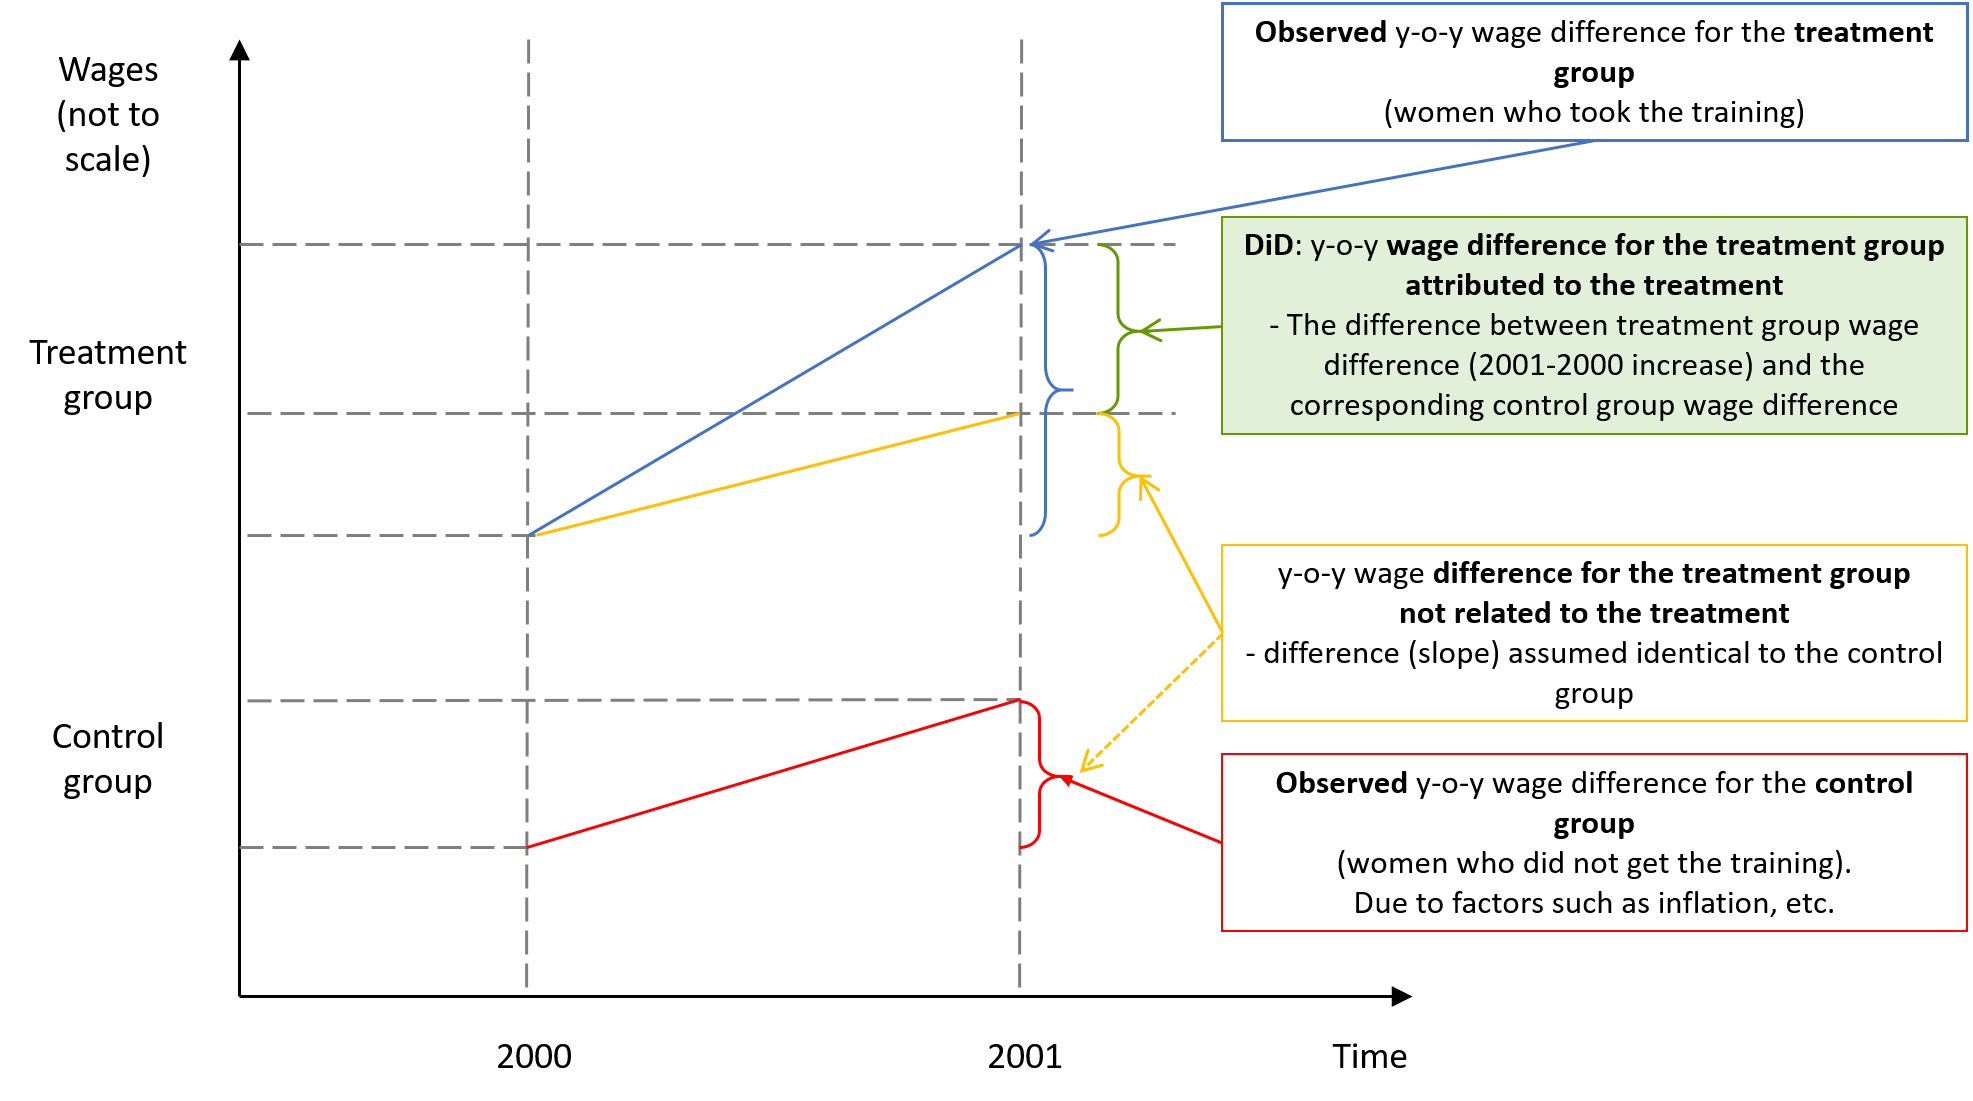
\includegraphics[width=\textwidth]{./IMG/Obrazek3}
\end{frame}
%---------------------------------
\begin{frame}{DiD estimator: Policy analysis with pooled CS data}
\small 
\underline{\textbf{DiD estimator:}} we use LRMs to compare changes in conditional means for the treatment and control groups.
\begin{itemize}
\item Group specific (treatment/control) and time specific effects are addressed.
\end{itemize}
\medskip
\underline{\textbf{Assumptions:}}
\begin{itemize}
\item Exogeneity of the treatment (of the $D_i$ variable): unbiased DiD estimates require that the treatment (individual being subject to economic policy change) is not systematically related to factors affecting the outcome (dependent variable), that are not accounted for explicitly in our model and thus are ``hidden'' in the random element.\\ \smallskip
\item DiD \textbf{attributes all differences in trends} between the treatment and control groups \textbf{to the intervention} (treatment). We assume there are no other factors that affect the difference in trends between the two groups.
\end{itemize}
\end{frame}
%---------------------------------
\begin{frame}{DiD estimator: Policy analysis with pooled CS data}
$$y_{it}=\beta_0 + \beta_1 D_i + \beta_2 T_t + \delta_1 (D_i T_t) + \varepsilon_{it}$$\\
\bigskip
\footnotesize
\begin{table}[]
\centering
\caption{Table: Illustration of the DiD estimator}\label{Tab1}
\begin{tabular}{|l|c|c|c|}
\hline
\multicolumn{1}{|c|}{$E(y_{it} | D_i, T_t)$} & Before $(t = 1)$    & After $(t=2)$                             & After -- Before        \\ \hline
Control $(D_i=0)$                                    & $\beta_0$           & $\beta_0 + \delta_0$                      & $\delta_0$            \\ \hline
Treatment $(D_i=1)$                                  & $\beta_0 + \beta_1$ & $\beta_0 + \delta_0 + \beta_1 + \delta_1$ & $\delta_0 + \delta_1$ \\ \hline
Treatment -- Control                        & $\beta_1$           & $\beta_1 + \delta_1$                      & \circled{$\delta_1$}            \\ \hline
\end{tabular}
\end{table} 

~\\
Again, if $\bm{x}_{it} \bm{\beta}$ is added back to the equation, interpretation of $\delta_1$ remains essentially unchanged.

\end{frame}
%---------------------------------
\begin{frame}{DiD estimator: Policy analysis with pooled CS data}
$$y_{it}=\beta_0 + \beta_1 D_i + \beta_2 T_t + \delta_1 (D_i T_t) + \varepsilon_{it}$$\\
\bigskip
In this simplified model (again, we drop $\bm{x}_{it} \bm{\beta}$), the estimated $\delta_1$ has \\a convenient DiD interpretation, as follows:\\
\bigskip
\begin{align*}
\hat{\delta}_1 &= (\overline{y}_{Tr,\,t=2} - \overline{y}_{Co,\,t=2}) -  (\overline{y}_{Tr,\,t=1} - \overline{y}_{Co,\,t=1}), \\ ~& \\
& \hspace{0.5cm} \textnormal{which may be rearranged as:} \\ ~& \\
&= (\overline{y}_{Tr,\,t=2} - \overline{y}_{Tr,\,t=1}) -  (\overline{y}_{Co,\,t=2} - \overline{y}_{\textit{Co},\,t=1}),
\end{align*}
where the \textit{Tr} subscript stands for treatment group and the \textit{Co} subscript identifies the control group.
\end{frame}
%---------------------------------
\begin{frame}{Example: DiD estimator}
\footnotesize{What is the effect of building garbage incinerator on housing prices?}
\scriptsize
\begin{table}[]
\centering
\label{Tab21}
\begin{tabular}{lclcc}
\multicolumn{3}{l}{Dependent Variable: RPRICE}                                          &                      & \multicolumn{1}{l}{}      \\
\multicolumn{3}{l}{Included observations: 321}                                          &                      & \multicolumn{1}{l}{}      \\
                                &                      & \multicolumn{1}{c}{}           &                      & \multicolumn{1}{l}{}      \\
\multicolumn{1}{c}{Variable}    & Coefficient          & \multicolumn{1}{c}{Std. Error} & t-Statistic          & \multicolumn{1}{l}{Prob.} \\
                                
                                & \multicolumn{1}{l}{} &                                & \multicolumn{1}{l}{} & \multicolumn{1}{l}{}      \\
\multicolumn{1}{c}{C}           & 82517.23             & \multicolumn{1}{c}{2726.910}   & 30.26034             & 0.0000                    \\
\multicolumn{1}{c}{Y81}         & 18790.29             & \multicolumn{1}{c}{4050.065}   & 4.639502             & 0.0000                    \\
\multicolumn{1}{c}{NEARINC}     & -18824.37            & \multicolumn{1}{c}{4875.322}   & -3.861154            & 0.0001                    \\
\multicolumn{1}{c}{Y81*NEARINC} & -11863.90            & \multicolumn{1}{c}{7456.646}   & -1.591051            & 0.1126                    \\
                                
                                & \multicolumn{1}{l}{} &                                & \multicolumn{1}{l}{} & \multicolumn{1}{l}{}      \\
R-squared                       & 0.173948             & \multicolumn{2}{l}{Mean dependent var}                & 83721.36                  \\
Adjusted R-squared              & 0.166131             & \multicolumn{2}{l}{S.D. dependent var}                & 33118.79                  \\
S.E. of regression              & 30242.90             & \multicolumn{2}{l}{Akaike info criterion}             & 23.48429                  \\
Sum squared resid               & 2.90E+11             & \multicolumn{2}{l}{Schwarz criterion}                 & 23.53129                  \\
Log likelihood                  & -3765.229            & \multicolumn{2}{l}{Hannan-Quinn criter.}              & 23.50306                  \\
F-statistic                     & 22.25107             & \multicolumn{2}{l}{Durbin-Watson stat}                & 1.557107                  \\
Prob(F-statistic)               & 0.000000             & \multicolumn{2}{l}{}                                  & \multicolumn{1}{l}{}     
\end{tabular}
\end{table}
\begin{tikzpicture}[<-,overlay,remember picture,inner sep=1.5pt,shorten <=0.2em,font=\footnotesize]
\tikzset{
    mynode/.style={rectangle,draw=blue, fill=blue!30, very thick, inner sep=.5em, minimum size=2em, text width=25em}
}
\node[mynode] at (7.8, 0.3) (Table){
\scriptsize{PRICE - house price in real terms (USD) \\ 
$Y81$ – dummy variable for $1981$, \ ($t=1978,1981$)\\
$1978$ – before ``rumors''~; $1981$ – incinerator operational \\
NEARINC – dummy for the treatment group}};
\end{tikzpicture}
\end{frame}
%---------------------------------
\begin{frame}{Example: DiD estimator}
\small
Incinerator effect on prices example, contd: \\
\medskip
The model may be easily expanded by explanatory variables such as: \textit{HOUSE.AGE, ROOMS, AREA, LOT.AREA}, etc. and the DiD interpretation remains basically unchanged \dots
\begin{block}{Selection bias (treatment effect vs. selection bias) example:}
\small
\textbf{Assumption:} “Unbiased DiD estimates require that the treatment is not systematically related to factors affecting the outcome that are not explicitly accounted for.”  \\
\medskip
Say, we have a “poor neighborhood” with relatively old and small houses and low house-prices. For complex reasons, it suffers from a representation deficit within the local city council (as compared to other “rich neighborhoods”) and is therefore more likely to get the incinerator. \\
\medskip
We do not have variables to control for this factor $\rightarrow$ the DiD estimator may be severely biased 
\end{block}

-- propensity to participation... as in Greene

\end{frame}
%---------------------------------
\section{Regression discontinuity design}
\begin{frame}{Regression discontinuity design}
    Violates common support assumption
\end{frame}
%---------------------------------
\section{Propensity score matching}
\begin{frame}{Propensity score matching}
    
\end{frame}
%---------------------------------





%---------------------------------
\begin{frame}{Treatment effects - additional literature}
\textbf{Treatment effects}\\
\medskip
For detailed \& technical discussion, see:\\
\medskip
\begin{itemize}
\item[1.] Greene: Econometric analysis, chapter 19.6
\medskip
\item[2.] Angrist, Pischke: Mostly Harmless Econometrics
\medskip
\item[3.] Cameron, Trivendi: Microeconometrics, Methods and Applications, chapter 25
\medskip
\item[4.] Wooldridge: Econometric analysis of C-S and panel data, chapter 21 Estimating Average Treatment Effects
\end{itemize}
\end{frame}
%---------------------------------
%---------------------------------------------------------------------
\end{document}